%% This file was auto-generated by IPython.
%% Conversion from the original notebook file:
%% eigseg2.ipynb
%%
\documentclass[11pt,english,fleqn]{article}

%% This is the automatic preamble used by IPython.  Note that it does *not*
%% include a documentclass declaration, that is added at runtime to the overall
%% document.

\usepackage{amsmath}
\usepackage{amssymb}
\usepackage{graphicx}
\usepackage{ucs}
\usepackage[utf8x]{inputenc}

% needed for markdown enumerations to work
\usepackage{enumerate}

% Slightly bigger margins than the latex defaults
\usepackage{geometry}
\geometry{verbose,tmargin=3cm,bmargin=3cm,lmargin=2.5cm,rmargin=2.5cm}

% Define a few colors for use in code, links and cell shading
\usepackage{color}
\definecolor{orange}{cmyk}{0,0.4,0.8,0.2}
\definecolor{darkorange}{rgb}{.71,0.21,0.01}
\definecolor{darkgreen}{rgb}{.12,.54,.11}
\definecolor{myteal}{rgb}{.26, .44, .56}
\definecolor{gray}{gray}{0.45}
\definecolor{lightgray}{gray}{.95}
\definecolor{mediumgray}{gray}{.8}
\definecolor{inputbackground}{rgb}{.95, .95, .85}
\definecolor{outputbackground}{rgb}{.95, .95, .95}
\definecolor{traceback}{rgb}{1, .95, .95}

% Framed environments for code cells (inputs, outputs, errors, ...).  The
% various uses of \unskip (or not) at the end were fine-tuned by hand, so don't
% randomly change them unless you're sure of the effect it will have.
\usepackage{framed}

% remove extraneous vertical space in boxes
\setlength\fboxsep{0pt}

% codecell is the whole input+output set of blocks that a Code cell can
% generate.

% TODO: unfortunately, it seems that using a framed codecell environment breaks
% the ability of the frames inside of it to be broken across pages.  This
% causes at least the problem of having lots of empty space at the bottom of
% pages as new frames are moved to the next page, and if a single frame is too
% long to fit on a page, will completely stop latex from compiling the
% document.  So unless we figure out a solution to this, we'll have to instead
% leave the codecell env. as empty.  I'm keeping the original codecell
% definition here (a thin vertical bar) for reference, in case we find a
% solution to the page break issue.

%% \newenvironment{codecell}{%
%%     \def\FrameCommand{\color{mediumgray} \vrule width 1pt \hspace{5pt}}%
%%    \MakeFramed{\vspace{-0.5em}}}
%%  {\unskip\endMakeFramed}

% For now, make this a no-op...
\newenvironment{codecell}{}

 \newenvironment{codeinput}{%
   \def\FrameCommand{\colorbox{inputbackground}}%
   \MakeFramed{\advance\hsize-\width \FrameRestore}}
 {\unskip\endMakeFramed}

\newenvironment{codeoutput}{%
   \def\FrameCommand{\colorbox{outputbackground}}%
   \vspace{-1.4em}
   \MakeFramed{\advance\hsize-\width \FrameRestore}}
 {\unskip\medskip\endMakeFramed}

\newenvironment{traceback}{%
   \def\FrameCommand{\colorbox{traceback}}%
   \MakeFramed{\advance\hsize-\width \FrameRestore}}
 {\endMakeFramed}

% Use and configure listings package for nicely formatted code
\usepackage{listingsutf8}
\lstset{
  language=python,
  inputencoding=utf8x,
  extendedchars=\true,
  aboveskip=\smallskipamount,
  belowskip=\smallskipamount,
  xleftmargin=2mm,
  breaklines=true,
  basicstyle=\small \ttfamily,
  showstringspaces=false,
  keywordstyle=\color{blue}\bfseries,
  commentstyle=\color{myteal},
  stringstyle=\color{darkgreen},
  identifierstyle=\color{darkorange},
  columns=fullflexible,  % tighter character kerning, like verb
}

% The hyperref package gives us a pdf with properly built
% internal navigation ('pdf bookmarks' for the table of contents,
% internal cross-reference links, web links for URLs, etc.)
\usepackage{hyperref}
\hypersetup{
  breaklinks=true,  % so long urls are correctly broken across lines
  colorlinks=true,
  urlcolor=blue,
  linkcolor=darkorange,
  citecolor=darkgreen,
  }

% hardcode size of all verbatim environments to be a bit smaller
\makeatletter 
\g@addto@macro\@verbatim\small\topsep=0.5em\partopsep=0pt
\makeatother 

% Prevent overflowing lines due to urls and other hard-to-break entities.
\sloppy

\setlength{\mathindent}{0pt}
\setlength{\parindent}{0pt}
\setlength{\parskip}{8pt}
\begin{document}

Ozdegerler ve Ozvektorler ile Imaj Bolmek, Gruplamak

Sentetik görüş (machine vision) dalında, karşımıza çıkan en temel
problemlerden biri, pikselleri guruplayarak bir nesneleyi tanımlamaktır.
Bildiğimiz gibi, robot gözden gelen sayısal bilgiler ışığında, 3-boyutlu
dünya bilgisayar için 2 boyutlu bir dünyaya dönüşür. Bu dünyada,
pikseller arasındaki bağlantı kaybolmuştur. Yani, elimizdeki veriye
tarafsız bir şekilde bakarsak, iki pikselin hangi nesneye ait olduğunu
belirten `gizli' bir kodlama bulmamız imkansızdır. İmgecikler arasında
yapmamız gereken bu bağlantıyı, algoritmalar kullanarak sonradan yapmaya
mecbur kalıyoruz. Yani, insan gözünün aynen yaptığı gibi.

İşte burada, guruplama (clustering) yöntemleri denen bir dizi algoritma
ve `düşünce şekli' yardımımıza yetişiyor. Çok temel bir konu olduğu
için, guruplama hakkında bir çok araştırmacı harıl harıl yeni
yaklaşımlar bulmak ile meşguller. Fakat daha hala tek bir kuram
diyebileceğimiz `hep işleyen' bir yaklaşım bulunabilmiş değil. Her
değişik ortam için, değişik guruplama yöntemleri kullanılıyor.

Her yöntemin başarı miktarı ötekine göre farklı. Burada özetleyeceğim
yöntem, doğrusal cebir ve çizge spektrum (spectrum) analizi yaparak
guruplamayı başarıyor. Bu kelimelerin anlamlarını aşağıda belirtelim.

Doğrusal cebir, matematik derslerinden hatırlayabileceğimiz gibi, üstü
olmayan bilinmezli denklemleri çözmenin aritmetiği demektir. Yani
doğrusal cebir denklemlerindeki bilinmeyenler, $x$, $y$, $z$ gibi
değerlerdir. $x^2$, $y^2$ gibi bilinmezlerle bu dalda uğraşılmaz.

Doğrusal cebir oldukca iyi araştırılmış ve kuramları yerine oturmuş bir
matematik dalıdır. Her ne kadar üniversitelerde analiz (calculus) dersi
kadar önem verilmese de, bilgisayarların daha güçlenmesi ile doğrusal
cebir daha da çok ragbet görür oldu. Doğrusal cebirin bizim icin ilginç
olan tarafı, son zamanlarda çizge kuramı (graph theory) ile kurulan
bağlantılarıdır. Yani, doğrusal cebirden bildiğimiz matris kavramının,
çizgeleri çözmek icin kullanılabilmesinin keşfedilmesi.

Bir sayısal görüntu ile çizge arasındaki bağlantı nedir diye merak
edebilirsiniz\ldots{} Daha sonra, çizge ile matris arasındaki bağlantı
nedir diye merak edilebilir\ldots{} Bu iki bağlantıyı teker teker
özetleyecegiz.

Daha rahat göz önüne getirebilmek için, aşağıdaki resme bakabiliriz.

\begin{codecell}
\begin{codeinput}
\begin{lstlisting}
im=imread("adjacency_graph.jpg"); imshow(im)
\end{lstlisting}
\end{codeinput}
\begin{codeoutput}
\begin{verbatim}
<matplotlib.image.AxesImage at 0xa71122c>
\end{verbatim}
\begin{center}
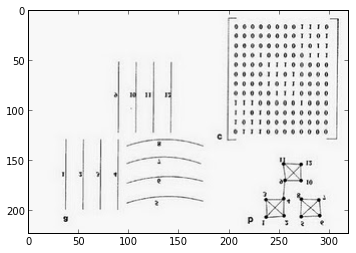
\includegraphics[width=0.7\textwidth]{eigseg2_files/eigseg2_fig_00.png}
\par
\end{center}
\end{codeoutput}
\end{codecell}
Bu resimde gördüğümüz (b) şeklinde görünen çizge, (a) şeklinde
gösterilen `ekrandaki' nesnelerin birbirine olan alakasına göre çizilmiş
bir çizgedir. Yani, (a) da görülen ner nesneyi (b) çizgesi üzerinde bir
düğüm noktası olarak belirtirsek, o zaman iki nesnenin birbiri ile,
herhangi bir ilişkisi durumunda, iki düğüm arasında bir bağlantı
kurarız. Bu işlemden sonra elimize gecen çizgeye bitişiklik çizgesi
diyoruz.

Bir çizge düğümler ve bunların arasındaki bağlantılardan ibârettir.

Cebire gelelim. Aynen doğrusal cebir de olduğu gibi, çizge üzerinde
kurulmuş bir kuram ve yöntem de var. Bu iki konu uzun sure ayrı yollarda
geliştiler ve râfine edildiler. Fakat yakın zamanda matematikçiler çizge
problemlerini çözmek için doğrusal cebir kullanmaya başladılar. Meselâ
bahsettiğimiz bitişiklik çizgesini `bitişiklik matrisine' çevirirsek,
doğrusal cebirin yontemlerini kullanarak, çizge hakkında bazı sonuçlara
varmamız mümkün oluyor. Bu çok ilginç ve harika bir bağlantı, ve bir
takim yapıcı yan etkileri var.

Bitişiklik matrisine örnek olarak (c) şekline bakabilirsiniz.

Bu matrisi yaratırken, her çizge üzerindeki her düğüme bir sayı
verdiğimizi unutmayalım; o zaman bu kodlamaya göre düğüm 1 ve düğüm 3
arasında bir ilişki var ise, matrise bakıp X ekseni = 1, ve Y ekseni = 3
üzerine tekâbül eden matris değerinin 1 olarak tanımlıyoruz.

Arasında ilişki olmayan düğümler, matris üzerinde 0 değeri taşıyorlar.

İşte bu matris üzerinde özdeğer, özvektör yöntemleri kullanarak çizge
hakkında sonuçlara varmak mümkün oluyor.

0 ve 1 degerleri yerine yakinligi piksel degerleri arasindaki farka
bagli olarak ta hesaplayabiliriz.

Gruplamak

Bir imaji nasil gruplara ayirabiliriz? Ekran piksellerini, çizge (graph)
düğümleri olarak gösterebiliriz, sonra bu çizgeyi yakinsallik (affinity)
matrisine çevirebiliriz. Bu matris üzerinde öyle işlemler yapalım ki,
elimize $Wx$ denen bir vektör geçsin; bu vektörün $1..N$ üyeleri, $1..N$
piksellerinin $x$ gurubuna üyelik katsayısı olsun. Katılım değerleri en
fazla olan vektör (gurup), ekran üzerindeki en büyük nesne demektir!

Matematiksel olarak şöyle bir formül kuralım, sadece temsil etmeye
ugraşıyoruz, yani bir gurup ve içinde olan pikseller arasında bağlantı
kurmak istiyoruz. Piksel ve herhangi bir gurup arasındaki ilişkiyi
formül ile kağıt üzerine dökmeyi amacliyoruz. Matematik, sayılar
arasında alâka kurma sanatıdır. Elimizde şimdilik bir algoritma olmasa
bile, temsili olarak bir alâka kurmak mümkün.
\[ \sum_{i=1}^n \sum_{j=1}^n w_{ij}x_ix_j = \mathbf{x}^T\mathbf{Ax} \]
Bu formüle göre, $Wij$, çizge üzerinde gösterilen i ve j düğümu
arasındaki bağlantı ağırlığı olacak. $x$ vektörünün içindeki her değer,
çizgedeki düğümlerin bu $x$ gurubuna dâhil olma katsayısı olacak.
Formülun sol tarafına göre, bu tanımları her i ve j değeri için yaparak
sonuçlarını toplamis oluyoruz.

Dikkat, toplam sonucu tek bir sayi, yani bir skalar. Nelerin birbiri ile
carpildigi optimizasyon icin cok onemli, $i$ ve $j$ arasindaki agirligi,
$i$'nin uyelik agirligi ve $j$'nin uyelik agirligi ile carpiyoruz,
bunlari tum diger kombinasyonlar icin yapiyoruz, ama bu carpimlari
topluyoruz. Carpim daha fazla buyutur, ve maksimizasyon icin bu buyukluk
daha on planda olacaktir.

Ve bu toplâmın `en büyük' olduğu yer, görüntü üzerindeki en büyük
nesnenin olduğu yerdir! Yâni elimizde bir matematiksel maksimizasyon
problemi var.

Caprimi tekrar kontrol edelim
\[ 
\left[\begin{array}{ccc}
a_1 & a_2 & a_3
\end{array}\right]
\left[\begin{array}{ccc}
b_{11} & b_{12} & b_{13} \\
b_{21} & b_{22} & b_{23} \\
b_{31} & b_{32} & b_{33} 
\end{array}\right]
\left[\begin{array}{c}
c_1 \\
c_2 \\
c_3
\end{array}\right]
 \]
Diyelim ki $i=2$, $j=1$. O zaman $a_2$, $b_{21}$ ve $c_1$'in birbiriyle
carpilmasi gerekir. Hakikaten caprimi elle kontrol edersek bunun
oldugunu gorecegiz. Icinde $a_1 \cdot b_{21}$ caprimini iceren terim,
sonra $c_1$ ile caprilacaktir.

Formülun yazarı, maksimizasyon işlemine atlamadan once, bir matematiksel
sınır daha koymaya mecbur olmuş. Maksimizasyon problemlerinde, her
sayıyı muazzam büyüklüklere getirerek formül sonucunu sürekli büyütmek
mümkün olabilirdi. Buna bir sınır getirmek için, sağ tarafta, A'nin
yanına çarpan olarak x vektörünün norm'u (yani uzunluğu) 1 olsun demiş.
Altta, bu tanımın açılmış halini görüyorsunuz. (Not: X vektörünün norm'u
= X'in devriği çarpı X). Lagrange formulu soyle gosterilebilir:
\[ w^TAw - \lambda (w^Tw - 1) \]\[ w^TAw - \lambda (w^Tw - 1) = 0\]\[ \frac{d}{dw} w^TAw - \lambda (w^Tw - 1) = 0 \]\[ 2Aw - 2\lambda w = 0\]\[ 2Aw = 2\lambda w \]\[ Aw = \lambda w \]
Ustteki son formul ozdeger (eigenvalue), ozvektorler (eigenvector)
formuludur. Rayleigh-Ritz kuramına göre, yukarıdaki formülün
enbuyütülmüş x vektörü , A matrisinin en buyuk özdeğerine tekabül eden
özvektör olacaktir! Dügümler birbirine ne kadar iyi bağlıysa, bir
gurubun içsel baglantısı ve `gurupluğu' o kadar iyi oluyor.

Bu son formül aşağıda
\[ \lambda_{n-k} = 
\max\limits_{x \perp x_{\lambda_n} , .... ,  x_{\lambda_{n-k+1}} } 
\mathbf{x}^T\mathbf{Ax}
\]
Ornek

Alttaki imaji gruplarina ayirmaya calisalim.

\begin{codecell}
\begin{codeinput}
\begin{lstlisting}
im=imread("twoObj.jpg"); imshow(im)

\end{lstlisting}
\end{codeinput}
\begin{codeoutput}
\begin{verbatim}
<matplotlib.image.AxesImage at 0xa92124c>
\end{verbatim}
\begin{center}
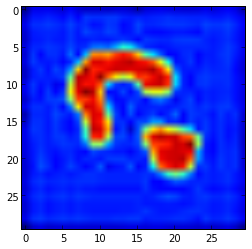
\includegraphics[width=0.7\textwidth]{eigseg2_files/eigseg2_fig_01.png}
\par
\end{center}
\end{codeoutput}
\end{codecell}
\begin{codecell}
\begin{codeinput}
\begin{lstlisting}
Img = plt.imread("twoObj.jpg")
n = Img.shape[0]
Img2 = Img.flatten(order='C')
nn = Img2.shape[0]

A = np.zeros((nn,nn))

for i in range(nn):
    for j in range(nn):
        A[i,j]=np.exp(-((Img2[i]-Img2[j])**2))
        
V,D = np.linalg.eig(A)
V = np.real(V)
a = np.real(D[0])

threshold = 0 # filter
a = np.reshape(a, (n,n))
Img[a<threshold] = 255
imshow(Img)


\end{lstlisting}
\end{codeinput}
\begin{codeoutput}
\begin{verbatim}
<matplotlib.image.AxesImage at 0xac4972c>
\end{verbatim}
\begin{center}
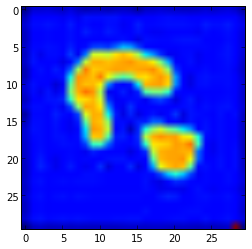
\includegraphics[width=0.7\textwidth]{eigseg2_files/eigseg2_fig_02.png}
\par
\end{center}
\end{codeoutput}
\end{codecell}
Kodda imread ile imaji okuduk, elimize 30x30 boyutunda bir matris gecti.
Bu matrisi once ``duzlestirerek'' bir vektor haline \# getirdik, ki bu
vektorun elemanlari yeni bir yakinlilik matrisinin kenarlari olacakti.
Sonra bu yeni elemanlarin her birini bir digeri ile karsilastirark
yakinligini hesapladik, bunu piksel degerinin ne kadar yakin olduguna
bakarak karar verdik, exp bunun icin kullanildi. Ayrica yakinlik ve
uzaklik kavramini tersine cevrildi, exp icinde eksi olmasi bundan,
birbirine ``benzer'' yani degerleri birbirine yakin olan piksellerin
farklari az olacaktir, fakat biz bu azligi maksimizasyon problemi icin
bir fazlaliga cevirmek istiyoruz.

Bu noktada A matrisinin ozdegerlerini hesaplattik, ve geriye C, D geri
geldi. Numpy ozdegerleri ve ona tekabul eden ozvektorleri buyukluk
sirasina dizerek geri getirir, bu sayede sifirini (ilk) D'ye bakarak en
buyuk ozdegere tekabul eden ozvektoru alabildik. Bu vektorun degerleri
ise uyeligi en yuksek olan grubu iceriyordu. Ciplak gozle bakinca bu
degerlerin uyelik icin pozitif, digerleri icin negatif degerler oldugunu
anladik, bu yuzden esik (threshold) degerini sifir olarak tanimladik.
Esigin altinda kalan degerleri grup disi olarak kabul ettik ve o
degerlerin kordinatina 255 piksel degerini atadik, ki ustteki resimde
mavi renkli gozuken pikseller bu degerleri temsil ediyor.

Kaynaklar

Sarkar ve Boyer makalesi ``Değisimlerin Sayısal Ölçümünü Özellik
Organizasyonu Kullanarak Yapmak: Özdeğerler ve Özvektörler''.
(Quantitative Measures of Change Based on Feature Organization:
EigenValues and EigenVectors)

Forsyth ve Ponce kitabı "Bilgisayar Görüşü, Yeni Yaklaşım (Computer
Vision, A Modern Approach)

\end{document}
